\begin{frame}{Restoration as an Inverse Problem}
  \begin{columns}[T,onlytextwidth]
    \column{0.54\textwidth}
      \begin{itemize}\footnotesize\itemsep0.35em
        \item \textbf{Observation model:} $y = \mathcal{A}(x) + n$, where $x$ is the clean image, $\mathcal{A}$ a degradation operator, $n$ noise, and $y$ the image we actually have.
        \item \textbf{One model, four tasks:} denoising ($\mathcal{A}$ is the identity), deblurring ($\mathcal{A}$ convolves with a blur kernel $k$), super-resolution or SR ($\mathcal{A}$ blurs, then keeps every $s$-th pixel in each direction), inpainting ($\mathcal{A}$ multiplies by a binary mask $m$).
        \item \textbf{Non-blind or blind:} a non-blind method is given $\mathcal{A}$ (the kernel, the noise level); a blind method must cope with an unknown $\mathcal{A}$. Photos from real cameras are the blind case.
        \item \textbf{Ill-posed:} $\mathcal{A}$ discards information. A $\times 4$ downsampling keeps $1/16$ of the pixels and a mask deletes them outright, so many different $x$ explain the same $y$.
        \item A learned restorer $f_\theta$ is trained on pairs $(x, \mathcal{A}(x)+n)$ built from clean images. Which of the many valid $x$ it returns is decided by its loss and by the prior it has learned.
      \end{itemize}
    \column{0.44\textwidth}
      \centering
      \vspace{0.3em}
      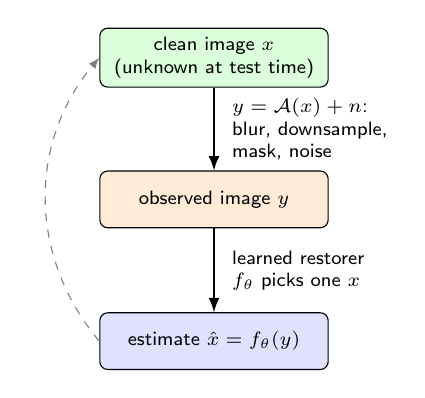
\begin{tikzpicture}[font=\sffamily\scriptsize, >=latex,
          blk/.style={draw, rounded corners=0.1cm, align=center, minimum width=2.9cm, minimum height=0.72cm},
          cln/.style={blk, fill=green!14}, obs/.style={blk, fill=orange!16}, est/.style={blk, fill=blue!12}]
        \node[cln] (x) at (0,3.6) {clean image $x$\\(unknown at test time)};
        \node[obs] (y) at (0,1.8) {observed image $y$};
        \node[est] (xh) at (0,0) {estimate $\hat{x} = f_\theta(y)$};
        \draw[->, thick] (x) -- node[right, align=left, xshift=0.1cm] {$y = \mathcal{A}(x) + n$:\\blur, downsample,\\mask, noise} (y);
        \draw[->, thick] (y) -- node[right, align=left, xshift=0.1cm] {learned restorer\\ $f_\theta$ picks one $x$} (xh);
        \draw[->, dashed, gray] (xh.west) to[bend left=40] (x.west);
      \end{tikzpicture}\\[0.3em]
      {\scriptsize Training pairs come from applying $\mathcal{A}$ to clean images; evaluation (dashed) compares $\hat{x}$ with the held-out $x$.\par}
  \end{columns}
\end{frame}

\begin{frame}{Fidelity Metrics: PSNR and SSIM}
  \begin{columns}[T,onlytextwidth]
    \column{0.52\textwidth}
      \begin{itemize}\footnotesize\itemsep0.3em
        \item \textbf{PSNR} (peak signal-to-noise ratio), in decibels:
        \[ \mathrm{PSNR} = 10 \log_{10} \frac{L^2}{\mathrm{MSE}}, \qquad \mathrm{MSE} = \frac{1}{N}\sum_{i=1}^{N} (x_i - \hat{x}_i)^2 \]
        $L$ is the peak pixel value (255 for 8-bit images) and $N$ the number of pixels. Halving the MSE adds about 3\,dB.
        \item \textbf{SSIM} (structural similarity) compares local means, contrasts and correlation:
        \[ \mathrm{SSIM}(x,\hat{x}) = \frac{(2\mu_x\mu_{\hat{x}} + C_1)(2\sigma_{x\hat{x}} + C_2)}{(\mu_x^2+\mu_{\hat{x}}^2+C_1)(\sigma_x^2+\sigma_{\hat{x}}^2+C_2)} \]
        $\mu$ and $\sigma^2$ are window means and variances, $\sigma_{x\hat{x}}$ the covariance, $C_1 = (0.01L)^2$ and $C_2 = (0.03L)^2$ keep the ratio stable. It is computed in $11 \times 11$ Gaussian windows ($\sigma = 1.5$) and averaged; 1 means identical.
      \end{itemize}
    \column{0.46\textwidth}
      {\footnotesize Image quality assessment (IQA) metrics come in three families:\par}
      \vspace{0.3em}
      {\centering\scriptsize\setlength{\tabcolsep}{3pt}
      \begin{tabular}{>{\raggedright\arraybackslash}p{1.35cm} >{\raggedright\arraybackslash}p{1.85cm} >{\raggedright\arraybackslash}p{2.25cm}}
        \toprule
        \textbf{Family} & \textbf{Examples} & \textbf{Rewards} \\
        \midrule
        Fidelity (needs $x$) & PSNR, SSIM & agreement with $x$ pixel by pixel, even if blurry \\
        \addlinespace[0.2em]
        Perceptual (needs $x$) & LPIPS, DISTS & similarity of deep features \\
        \addlinespace[0.2em]
        No-reference & NIQE, MUSIQ, MANIQA, CLIP-IQA, Q-Align & looking natural, with no access to $x$ \\
        \bottomrule
      \end{tabular}\par}
      \vspace{0.3em}
      \begin{itemize}\scriptsize\itemsep0.2em
        \item Most SR papers compute PSNR and SSIM on the luminance (Y) channel of the YCbCr colour space.
        \item \textbf{Q-Align} (ICML 2024) teaches a multimodal LLM to answer with five words, from \emph{excellent} to \emph{bad}; the score is the probability-weighted average of the five levels.
      \end{itemize}
  \end{columns}
  \vspace{0.2em}
  {\scriptsize SSIM: Wang et al., ``Image Quality Assessment: From Error Visibility to Structural Similarity,'' \textit{IEEE TIP} 13(4), 2004, \href{https://doi.org/10.1109/TIP.2003.819861}{doi:10.1109/TIP.2003.819861}, Eq.~13. Families as grouped in Wu et al., \href{https://arxiv.org/abs/2406.08177v3}{arXiv:2406.08177v3}, Sec.~4.1, which also reports the distribution-level FID. Q-Align: Wu et al., \href{https://arxiv.org/abs/2312.17090}{arXiv:2312.17090}.\par}
\end{frame}

\begin{frame}{The Perception-Distortion Trade-off}
  \begin{columns}[T,onlytextwidth]
    \column{0.53\textwidth}
      \begin{itemize}\footnotesize\itemsep0.35em
        \item \textbf{Distortion} $\mathbb{E}[\Delta(X,\hat{X})]$: average dissimilarity to the true image (MSE, SSIM, \ldots). \textbf{Perception} $d(p_X, p_{\hat{X}})$: divergence between the distribution of outputs and that of natural images, i.e.\ how easily outputs are told apart from real photos.
        \item Blau and Michaeli define the best perception reachable at distortion $D$:
        \[ P(D) = \min_{p_{\hat{X}|Y}} d(p_X, p_{\hat{X}}) \;\; \text{s.t.} \;\; \mathbb{E}[\Delta(X,\hat{X})] \leq D \]
        and prove $P(D)$ is non-increasing, and convex when $d$ is convex in its second argument, for \emph{any} distortion measure $\Delta$. Below the curve is unreachable.
        \item The minimum-MSE (MMSE) estimate averages all plausible $x$. An average of valid images is usually not a valid image, so the result is blurry.
        \item Near the curve, lowering distortion costs perceptual quality and vice versa: report one fidelity and one perceptual metric together.
      \end{itemize}
    \column{0.45\textwidth}
      \centering
      \vspace{0.4em}
      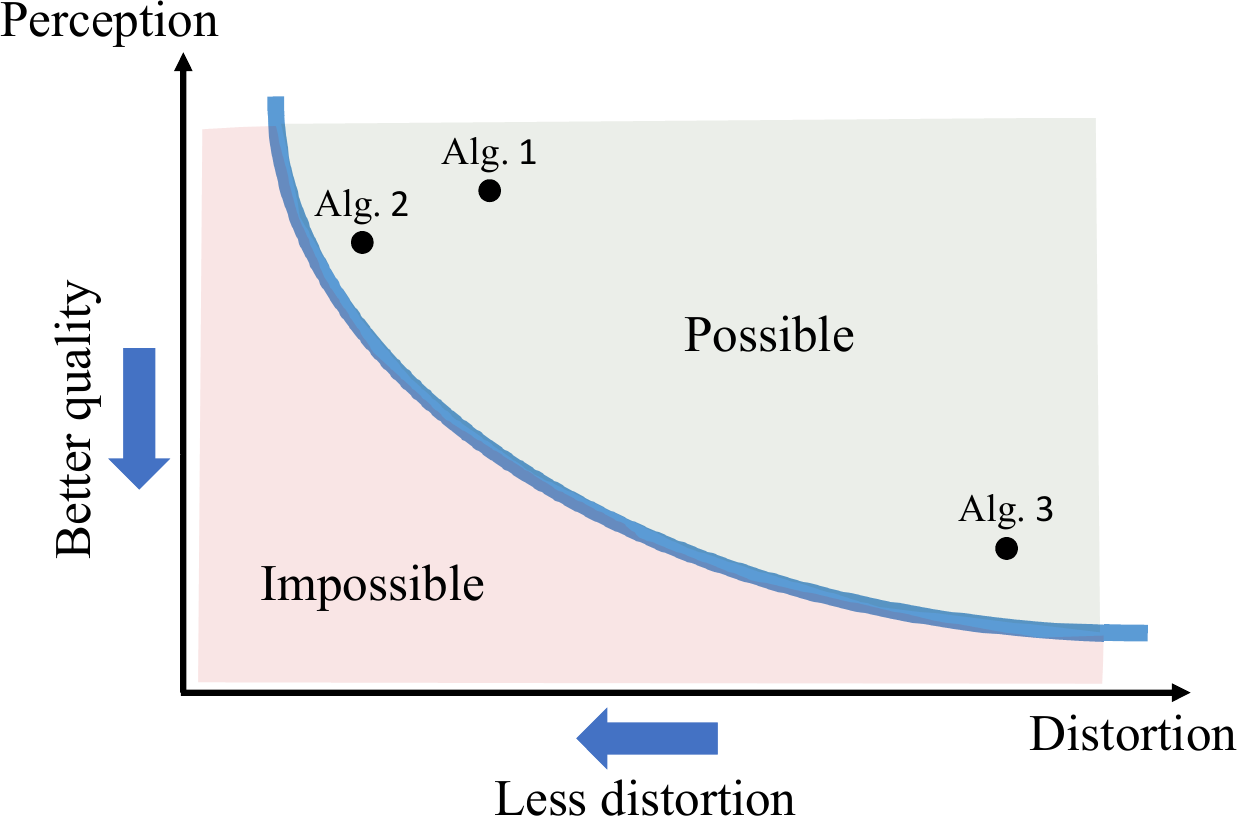
\includegraphics[width=\linewidth,height=0.55\textheight,keepaspectratio]{images/image-restoration-applications/blau_fig1_perception_distortion_plane.png}\\[0.2em]
      {\scriptsize Blau \& Michaeli, ``The Perception-Distortion Tradeoff,'' CVPR 2018, \href{https://arxiv.org/abs/1711.06077v2}{arXiv:1711.06077v2}, Definition~1, Theorem~1, Figure~1.\par}
  \end{columns}
\end{frame}

\begin{frame}{The Trade-off in Real Super-Resolution Models}
  \centering
  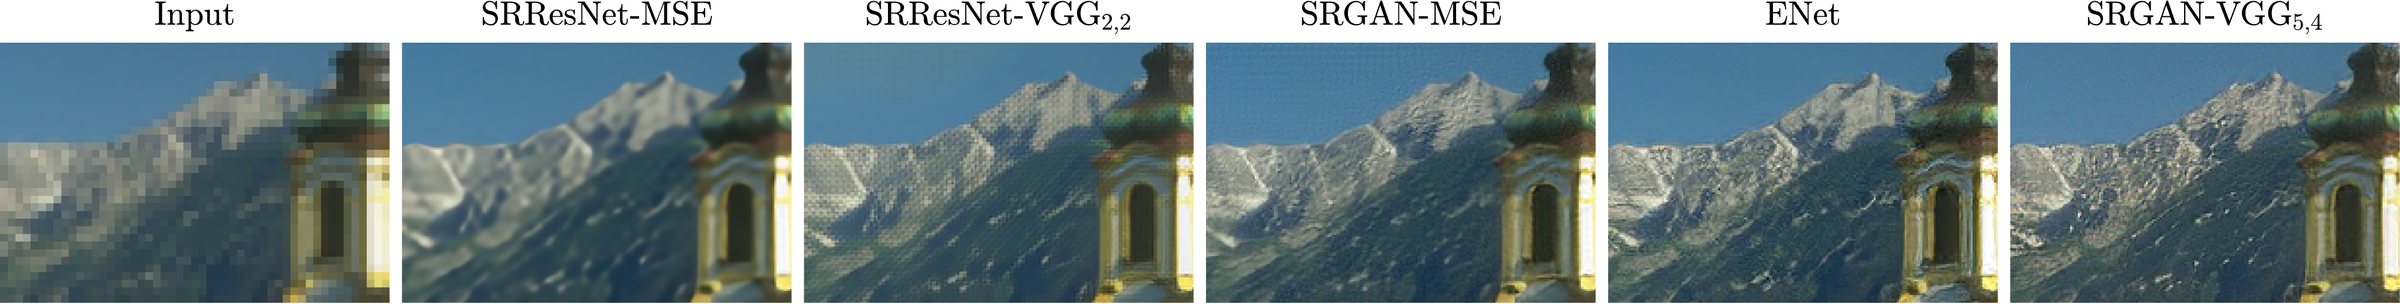
\includegraphics[width=\textwidth,height=0.25\textheight,keepaspectratio]{images/image-restoration-applications/blau_fig9_sr_low_to_high_distortion.png}\\[0.1em]
  {\scriptsize $\times 4$ SR outputs ordered from low to high distortion. Blau \& Michaeli, \href{https://arxiv.org/abs/1711.06077v2}{arXiv:1711.06077v2}, Figure~9.\par}
  \vspace{0.3em}
  \begin{columns}[T,onlytextwidth]
    \column{0.42\textwidth}
      \centering
      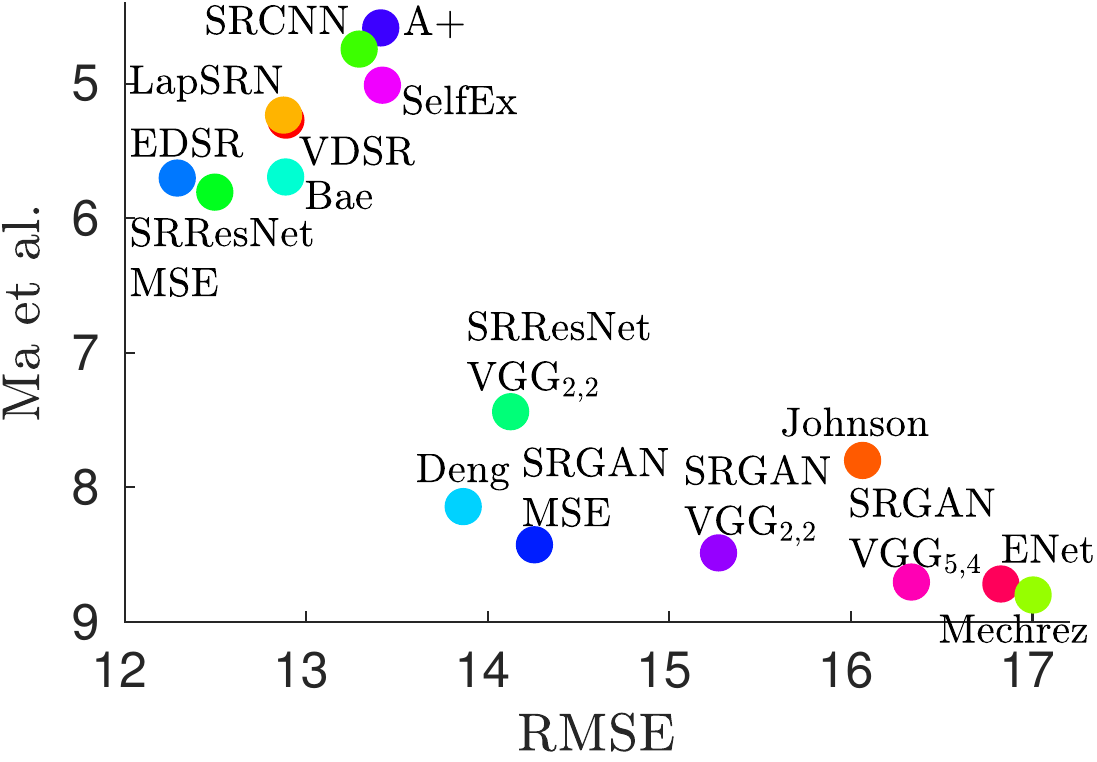
\includegraphics[width=\linewidth,height=0.46\textheight,keepaspectratio]{images/image-restoration-applications/blau_fig8a_sr_methods_rmse_vs_perception.png}\\[0.1em]
      {\scriptsize Same paper, Figure~8, panel for root-mean-square error (RMSE).\par}
    \column{0.56\textwidth}
      \begin{itemize}\footnotesize\itemsep0.35em
        \item 16 SR methods on BSD100 at $\times 4$. Lower on the vertical axis (a no-reference quality score) is perceptually better.
        \item The lowest-RMSE models sit in the perceptually poor upper-left cluster; those trained with adversarial or deep-feature losses score best perceptually and sit far to the right on RMSE. The empty lower-left corner is the unreachable region.
        \item A network trained with $\ell_{\mathrm{MSE}} + \lambda\,\ell_{\mathrm{adv}}$ moves along the curve as $\lambda$ grows (shown in the paper for a denoiser, Figure~6).
        \item The diffusion-prior restorers that follow aim at the perceptual end of this curve.
      \end{itemize}
  \end{columns}
\end{frame}

\begin{frame}{Synthetic Degradations for Real Photos}
  \centering
  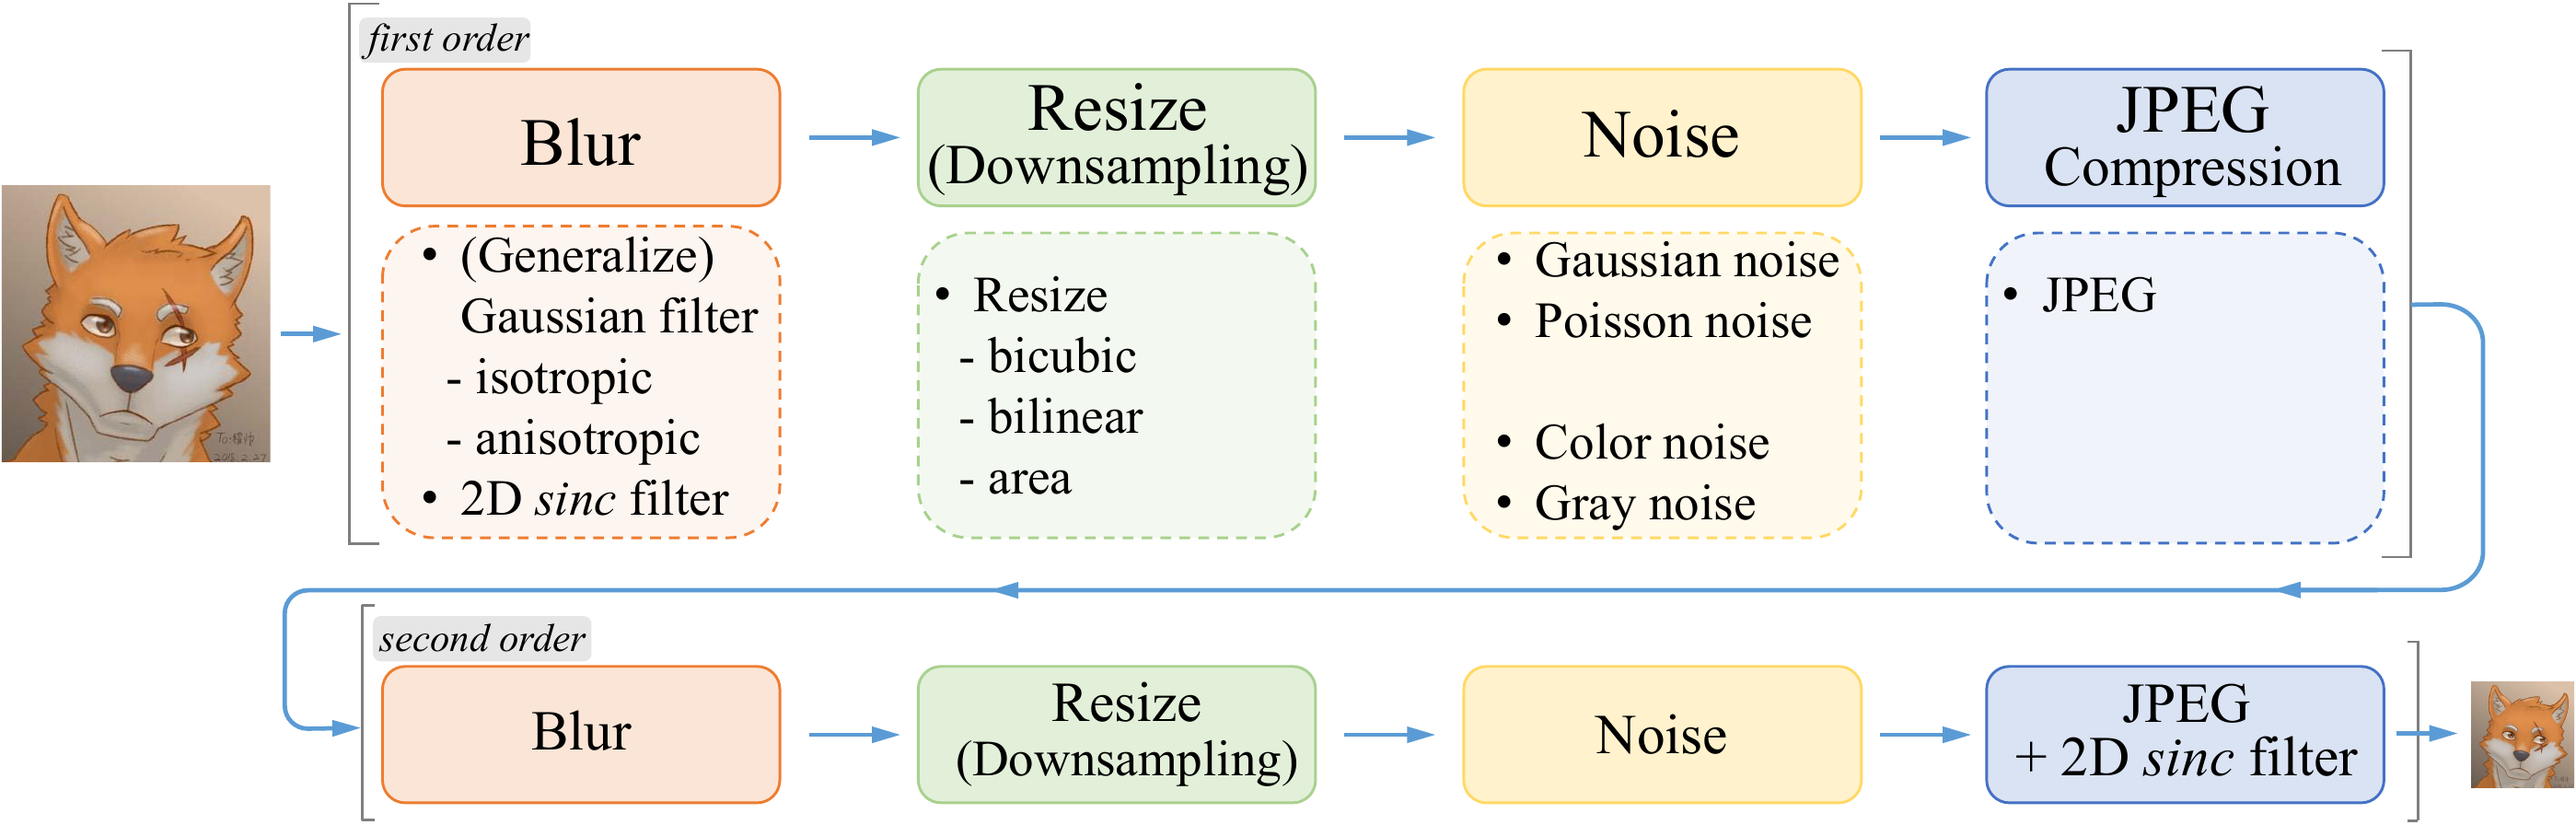
\includegraphics[width=\textwidth,height=0.34\textheight,keepaspectratio]{images/image-restoration-applications/realesrgan_fig2_second_order_degradation.png}\\[0.1em]
  {\scriptsize Wang et al., ``Real-ESRGAN: Training Real-World Blind Super-Resolution with Pure Synthetic Data,'' ICCV Workshops 2021, \href{https://arxiv.org/abs/2107.10833v2}{arXiv:2107.10833v2}, Figure~2; repositories \href{https://github.com/xinntao/Real-ESRGAN}{xinntao/Real-ESRGAN}, \href{https://github.com/xinntao/Real-ESRGAN-ncnn-vulkan}{xinntao/Real-ESRGAN-ncnn-vulkan} and \href{https://github.com/upscayl/upscayl}{upscayl/upscayl}.\par}
  \vspace{0.2em}
  \begin{columns}[T,onlytextwidth]
    \column{0.49\textwidth}
      \begin{itemize}\footnotesize\itemsep0.3em
        \item Classic SR models assume ideal bicubic downsampling; real photos carry camera blur, sensor noise, resizing and repeated JPEG compression, so the mismatch breaks them.
        \item Classical model: $y = \big[(x \ast k)\!\downarrow_s + \, n\big]_{\mathrm{JPEG}}$ (Eq.~1, in this lecture's notation). Models trained on it still amplify noise and ringing on complex photos (Figure~3), so Real-ESRGAN applies it \textbf{twice} with random blur, resize, Gaussian or Poisson noise and JPEG quality, plus sinc filters for ringing.
      \end{itemize}
    \column{0.49\textwidth}
      \begin{itemize}\footnotesize\itemsep0.3em
        \item Still the default: SUPIR, OSEDiff, InvSR, TSD-SR, DreamClear, DiT4SR and LucidFlux, 2024--2026 diffusion restorers, all synthesise their training pairs with this pipeline.
        \item Also a widely used local upscaler: its portable ncnn-vulkan executables run on Intel, AMD and Nvidia GPUs without CUDA or PyTorch (MIT; the PyTorch code is BSD-3-Clause), and the Upscayl desktop app is built on it (AGPL-3.0).
      \end{itemize}
  \end{columns}
\end{frame}
